% !TEX root = /Users/kartikgohil/Documents/Imperial/Year4/Project/Docs/Final_Report/report_tex/main.tex
\section{Appendices}
\appendix

\section{Circuit Diagrams} \label{Circuit Diagrams}


\subsection{Circuit Diagram for HC-06 to Arduino Connection}
\label{arduinobluetooth}
\begin{figure}[H]
\centering
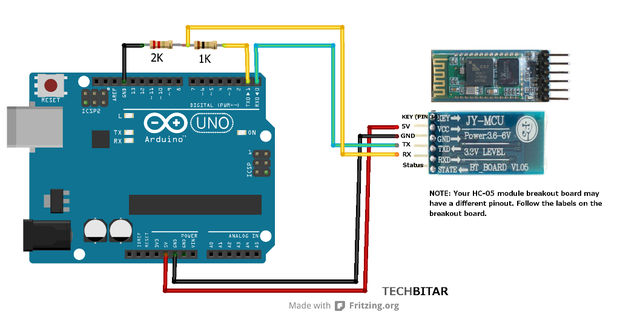
\includegraphics[scale = 1]{Images/arduinobluetooth}
\caption*{Image Available from Reference~\cite{arduinobluetooth}}
\end{figure}

\subsection{Circuit Diagram for Prototype 0.2.03 - Finger Board}
\label{fingerboardsch}
\begin{figure}[H]
\centering
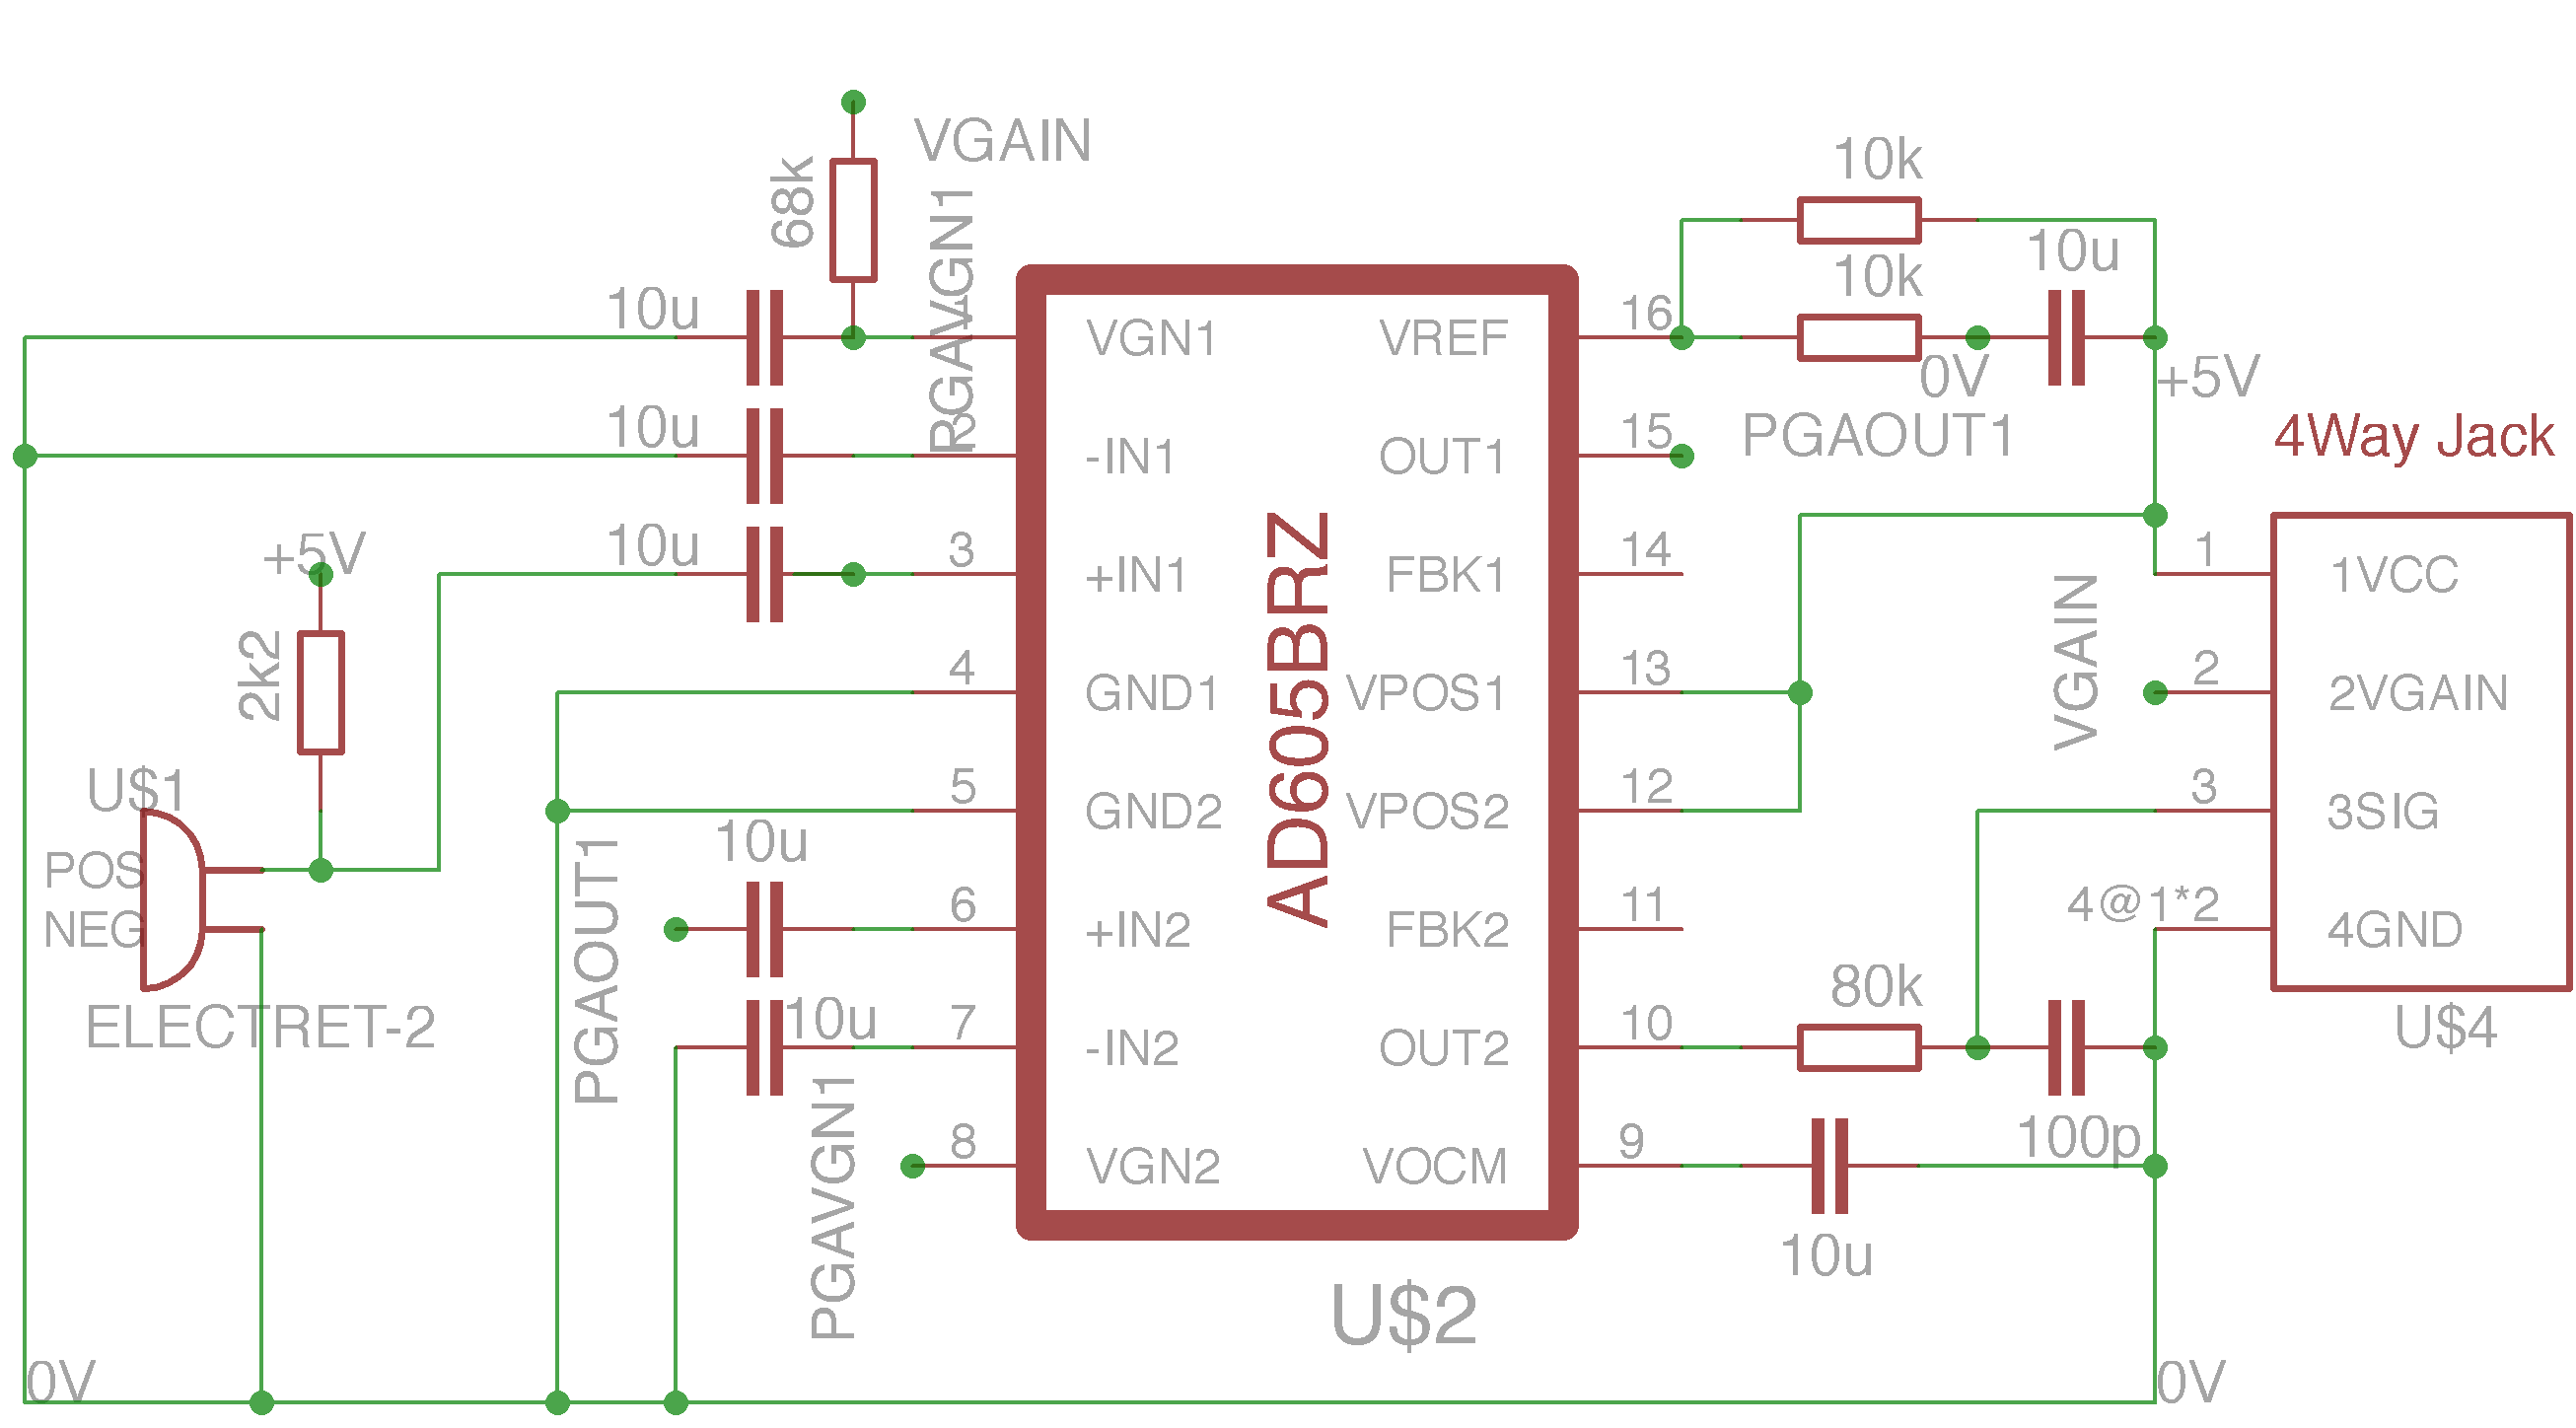
\includegraphics[scale = 1]{Images/mic_schematic_01}
\end{figure}

\subsection{Circuit Diagram for Prototype 0.2.03 - Arduino Shield}
\label{ardshieldsch}
\begin{figure}[H]
\centering
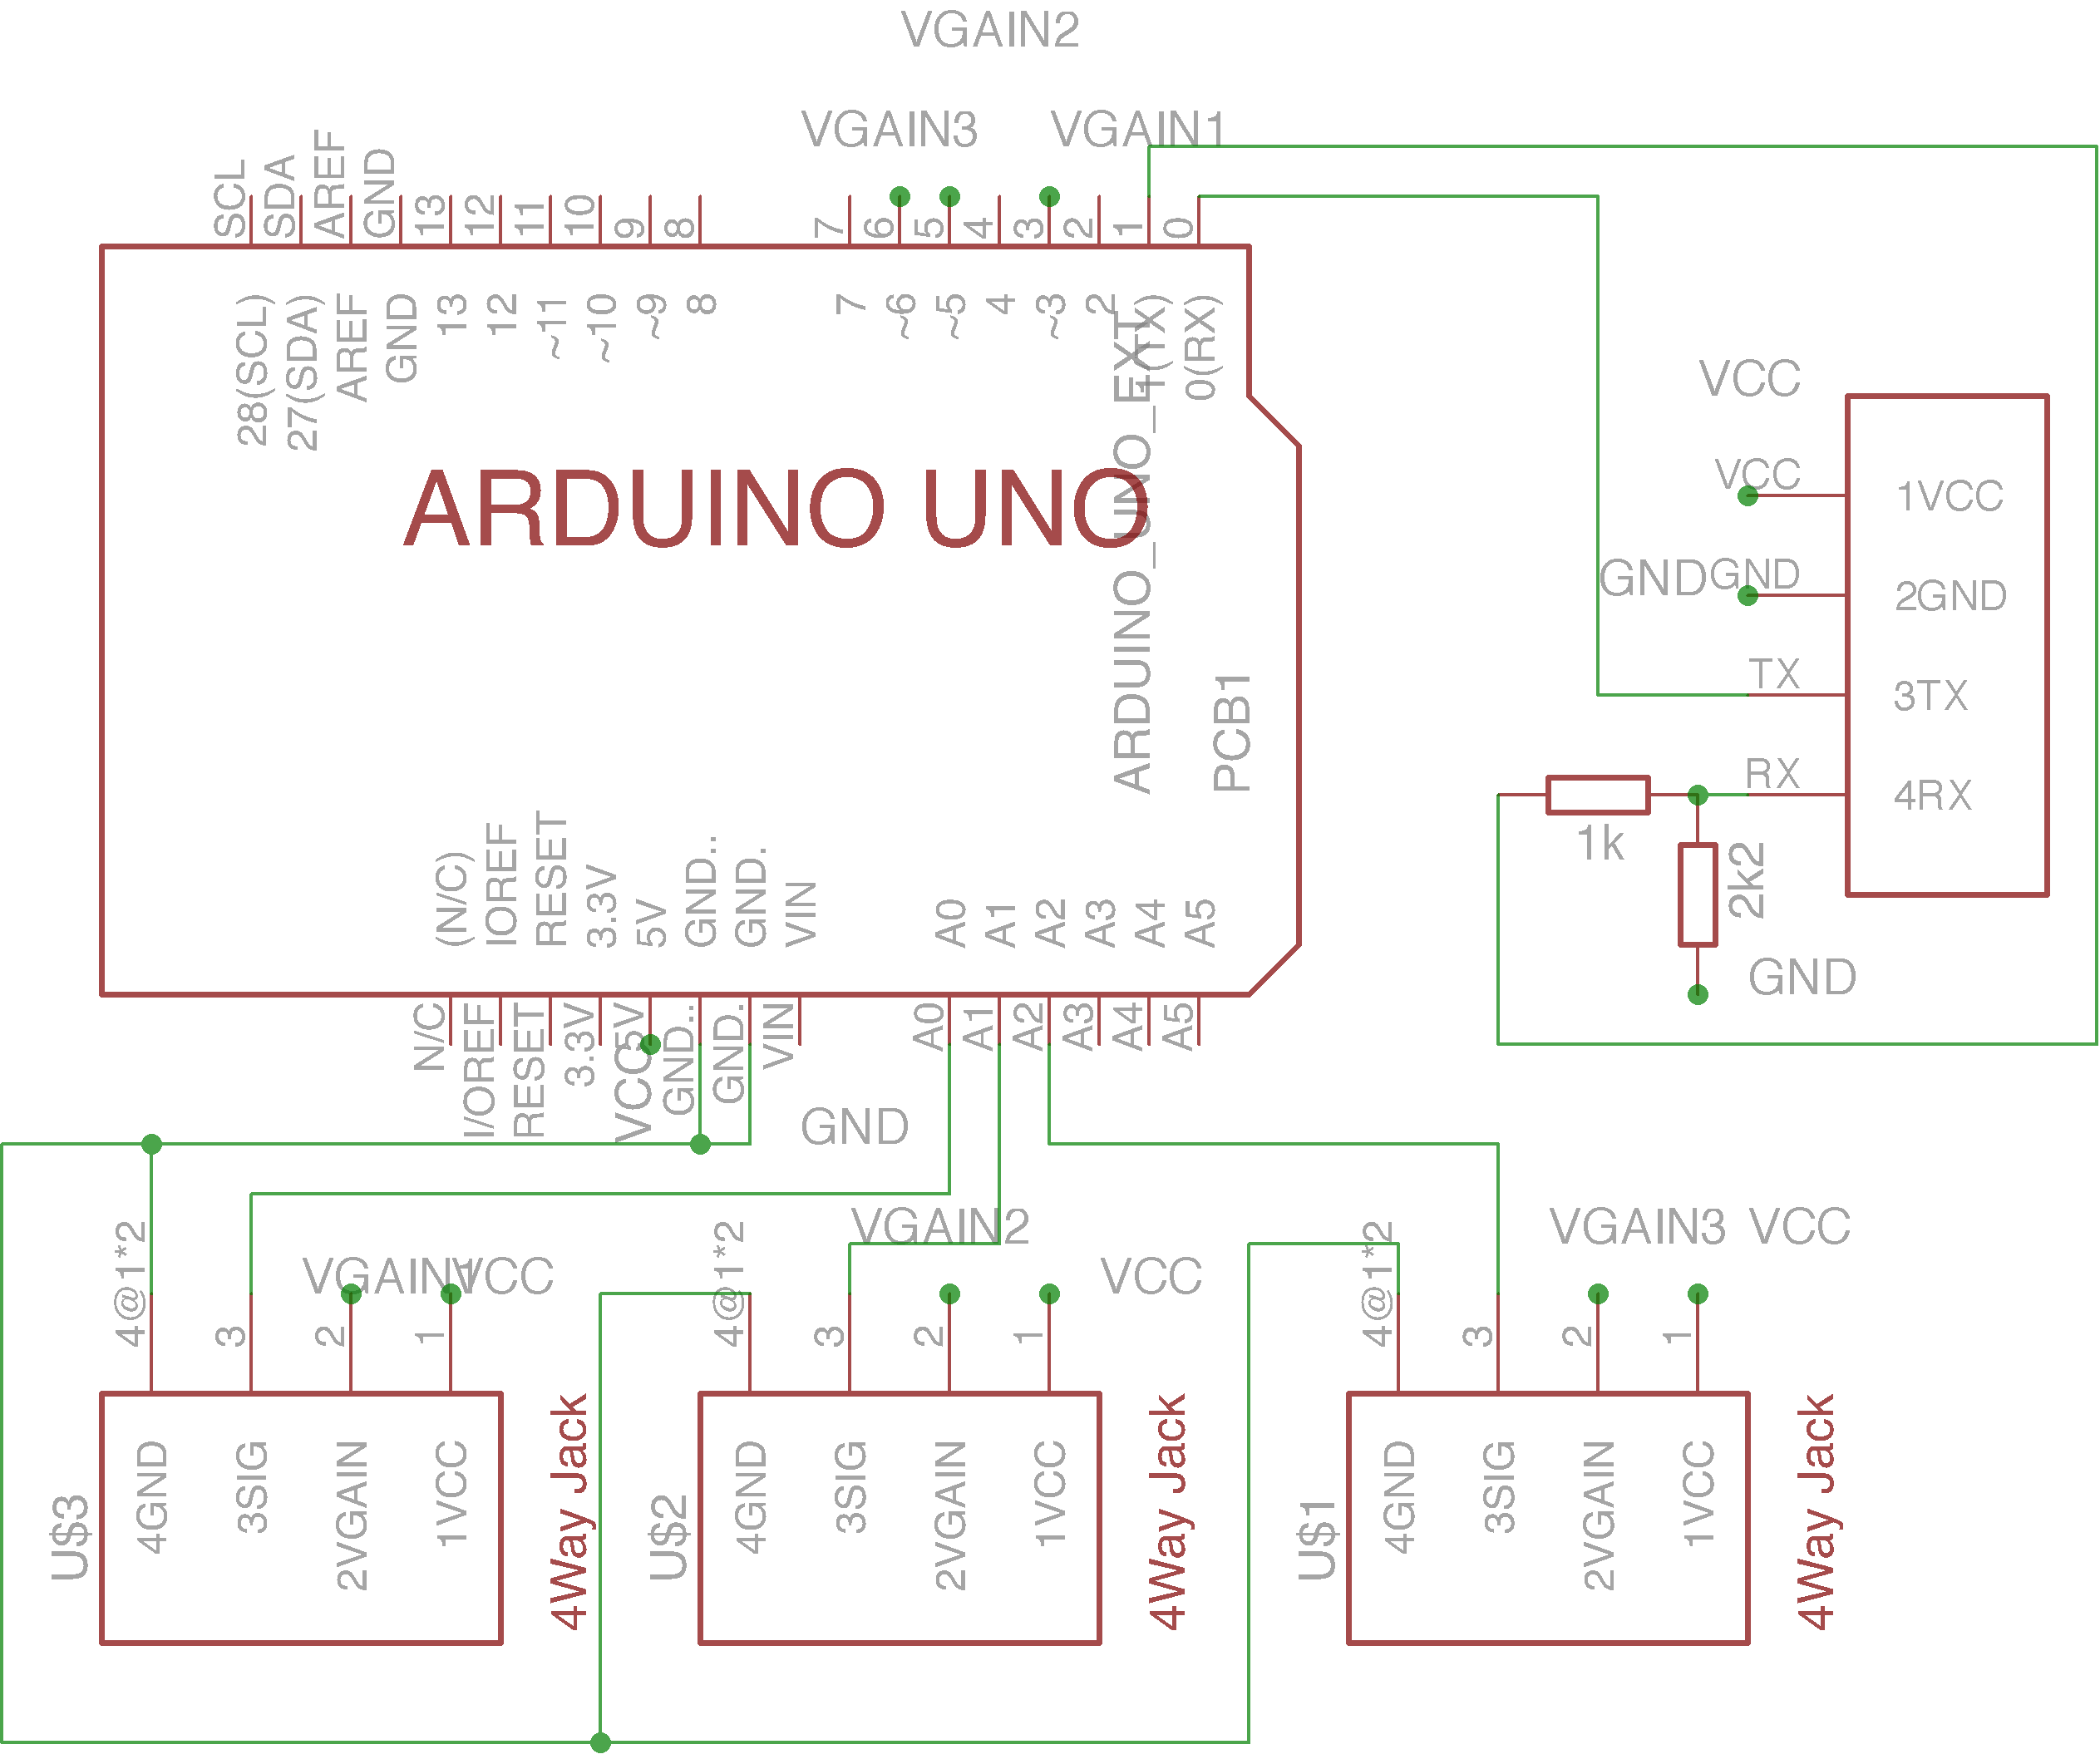
\includegraphics[scale = 1]{Images/ard_schematic_01}
\end{figure}



\section{Flow Diagrams} \label{Flow Diagrams}

\subsection{Flow Diagram for Microcontroller Program, Prototype 0.1.01}
\label{mcflow}
\begin{figure}[H]
\centering
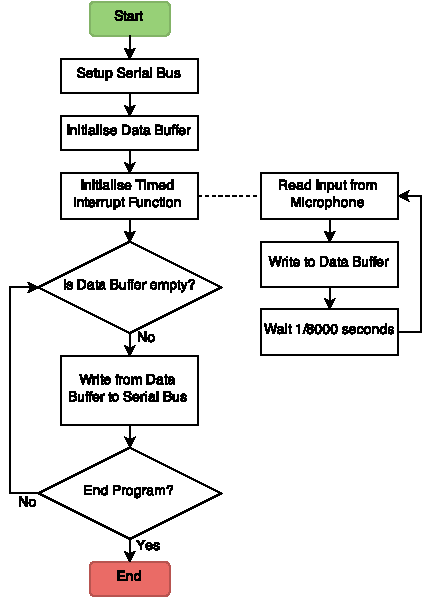
\includegraphics[scale = 1]{Images/mc0101}
\end{figure}


\newpage
\subsection{Flow Diagram for Interface Program, Prototype 0.1.01}
\label{interfaceflow}
\begin{figure}[H]
\centering
\subfloat[Voice Function Program]{
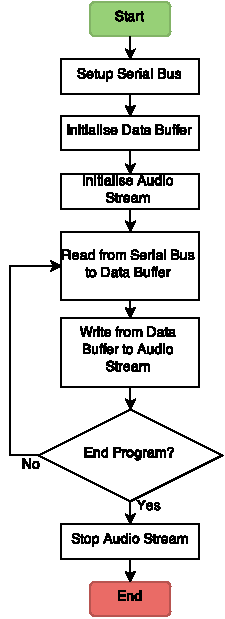
\includegraphics[scale = 1]{Images/interfacevoiceflow}
}
\hspace{72pt}
\subfloat[Sample Function Program]{
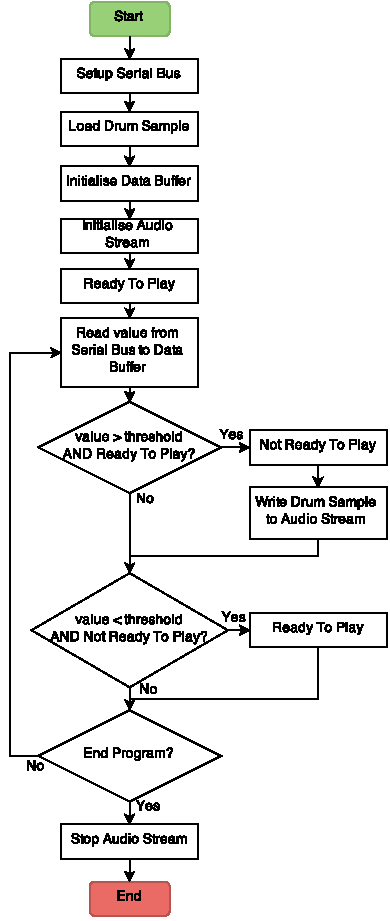
\includegraphics[scale = 1]{Images/interfacesampleflow}
}
\end{figure}

\subsection{Flow Diagram for Interface Program, Prototype 0.1.02}
\label{pyblue_flow}
\begin{figure}[H]
\centering
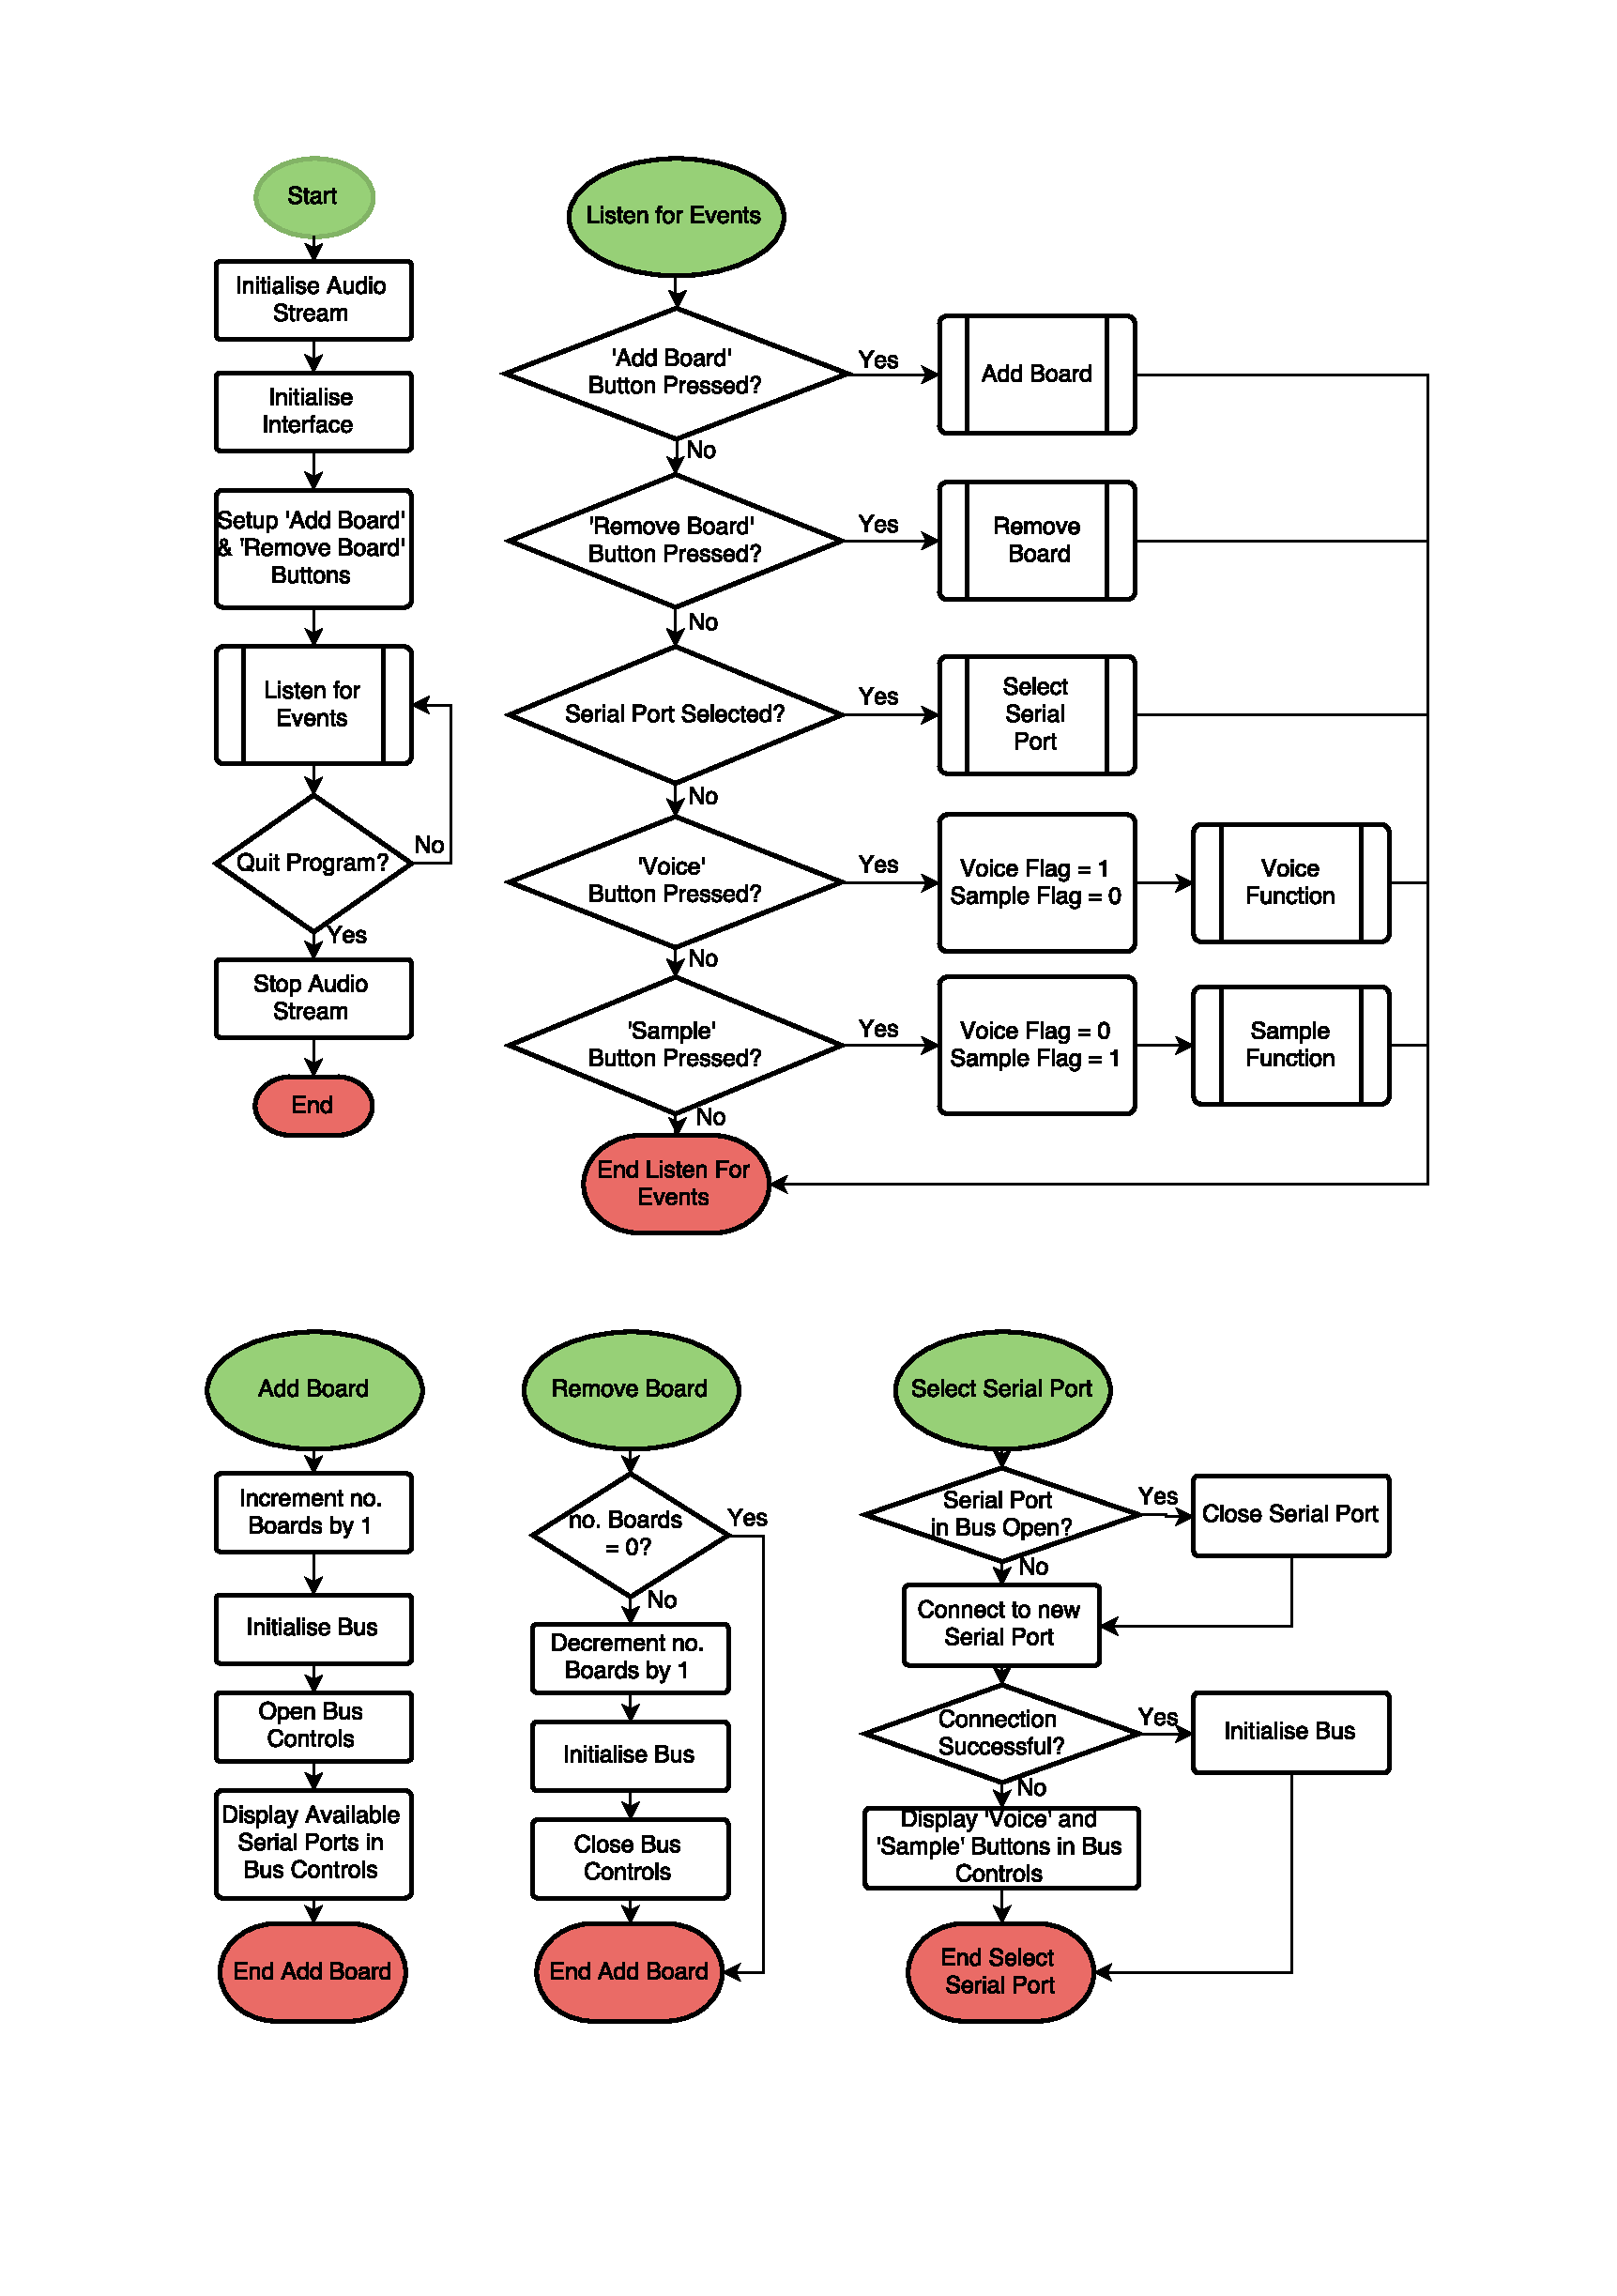
\includegraphics[scale = 0.7]{Images/PyFlow}
\end{figure}

\subsection{Flow Diagram for Interface Program, Prototype 0.2.01}
\label{juceflow}
\begin{figure}[H]
\centering
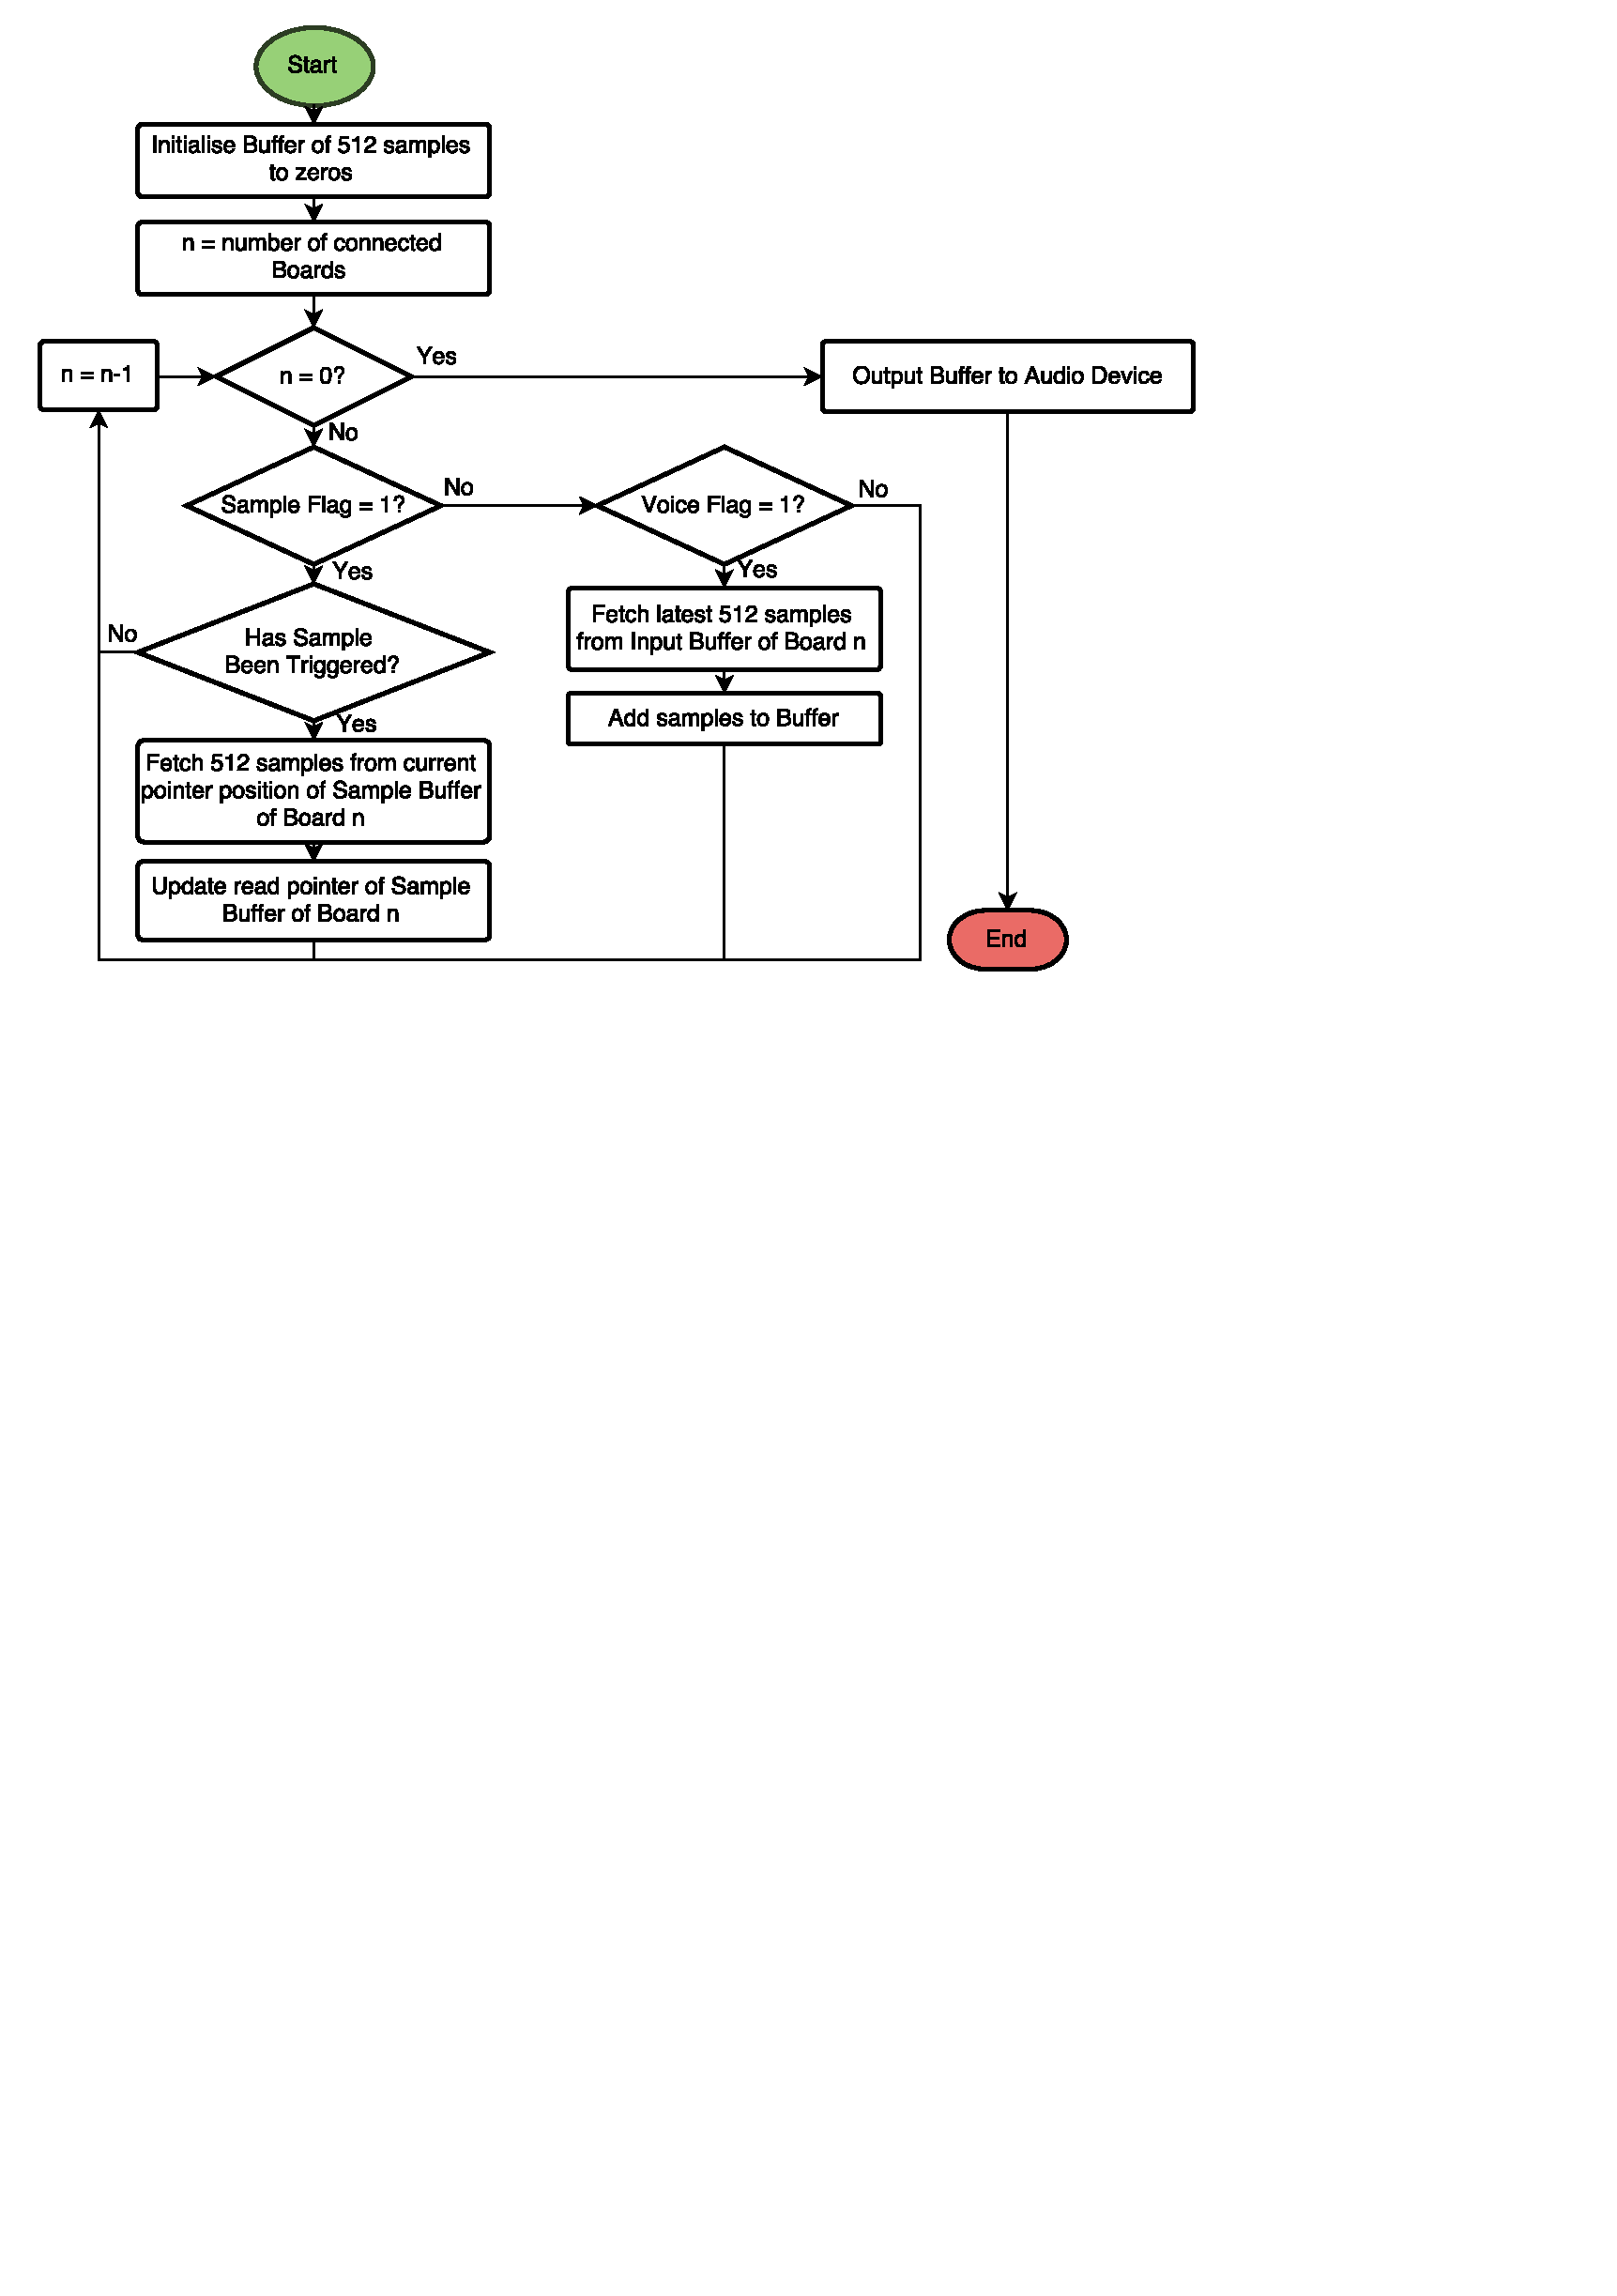
\includegraphics[scale=0.7]{Images/JuceFlow}\\
Function Diagram of Audio Transfer between storage buffers for each connected Board and the audio device.
\end{figure}


\section{PCB Design}

\subsection{Finger Board}
\label{fingerboardpcb}
\begin{figure}[H]
\centering
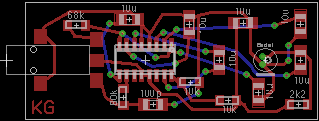
\includegraphics[scale = 2]{Images/mic_pcb_02}
\\ Dimensions: 49.51 x 19.99 mm
\end{figure}

\subsection{Arduino Shield Version 1}
\label{ardshieldpcb}
\begin{figure}[H]
\centering
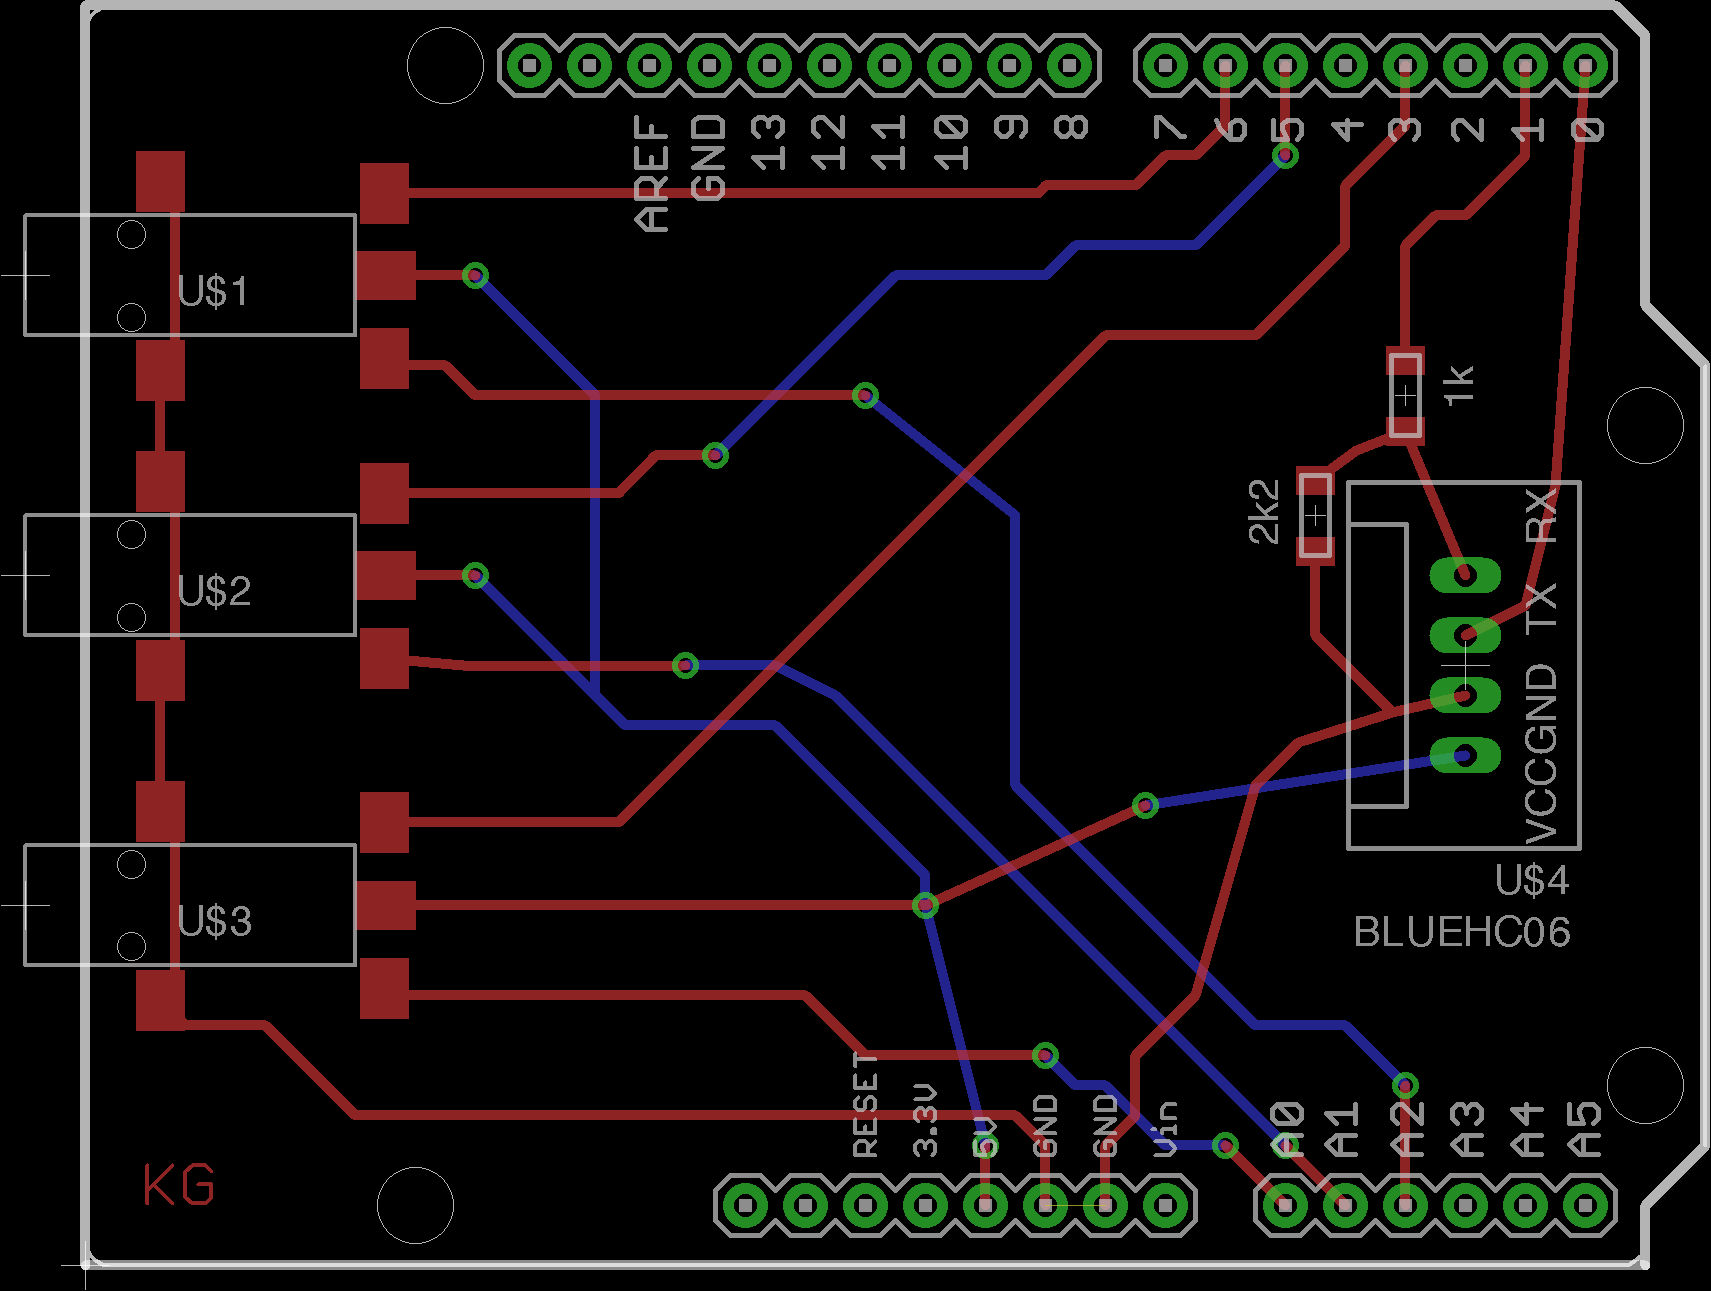
\includegraphics[scale = 1.5]{Images/ard_pcb_01}
\\ Dimensions: 68.58 x 53.34 x 2.5mm
\end{figure}

\subsection{Arduino Shield Version 2}
\label{ardshieldpcb2}
\begin{figure}[H]
\centering
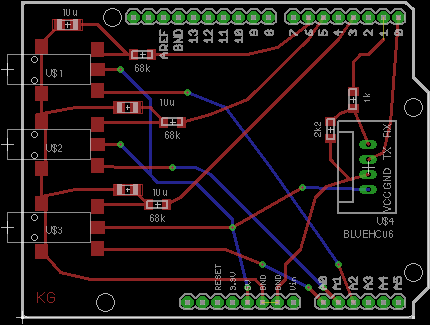
\includegraphics[scale = 1.5]{Images/ard_pcb_02}
\\ Dimensions: 68.58 x 53.34 x 2.5mm
\end{figure}







